\documentclass{article}

\usepackage[utf8]{inputenc}
\usepackage{enumitem}
\usepackage{todonotes}
\usepackage[ngerman]{babel}
\usepackage{amsmath}
\usepackage{booktabs}
\usepackage{float}

\DeclareMathOperator{\sgn}{sgn}

\title{Blatt 8}
\author{Luca Krüger, Jonas Otto, Jonas Merkle (Gruppe R)}
\date{\today}

\begin{document}
\maketitle

\section{Momentum Optimierer}
\begin{enumerate}[label=\arabic*.]
  \item
        \begin{align*}
          m(0) & = 0   & w(0) & = 20 \\
          m(1) & = 80  & w(1) & = 12 \\
          m(2) & = 120 & w(2) & = 0  \\
        \end{align*}
  \item Beschleunigung/Stabilisierung
        \begin{figure}[H]
          \centering

          \begin{tabular}{c|cc}
            \toprule
                                                                 & $\displaystyle \frac{\partial E}{\partial w(1)} < 0$ & $\displaystyle \frac{\partial E}{\partial w(1)} > 0$ \\
            \midrule
            $\displaystyle \frac{\partial E}{\partial w(0)} < 0$ & +                                                    & $-$                                                  \\
            $\displaystyle \frac{\partial E}{\partial w(0)} > 0$ & $-$                                                  & +                                                    \\
            \bottomrule
          \end{tabular}
        \end{figure}

  \item
        \begin{enumerate}[label=\alph*)]
          \item $m(t)$ ist durch seine rekursive Definition über $m(t-1)$ und den Gradienten $\frac{\partial E}{\partial w(t-1)}$ eine Differentialgleichung zweiter Ordnung. $m(t)$ ist daher eine (in unserem Fall gedämpfte) Schwingung. Die Gewichte $w(t)$ hängen direkt von $m(t)$ ab. Dadurch ist ein Überschwingen des Pfades von $w(t)$ in Abhängigkeit der gewählten Parameter $\eta, \alpha$ und der Startwerte $w(0), m(0)$ möglich.
          \item $m(t)$ zeigt wie der Gradient $\frac{\partial E}{\partial w(t-1)}$ in die Richtung des größten Anstieges. \\
                Die Gewichte $w(t)$ sollen aber in Richtung des kleinsten Anstieges optimiert werden, weshalb $m(t)$ mit negativem Vorzeichen in der Definition von $w(t)$ vorkommt.
          \item Oszillationen treten z.B. auf, wenn der Parameter $\alpha$ groß gewählt wird:
                \begin{figure}[H]
                  \centering
                  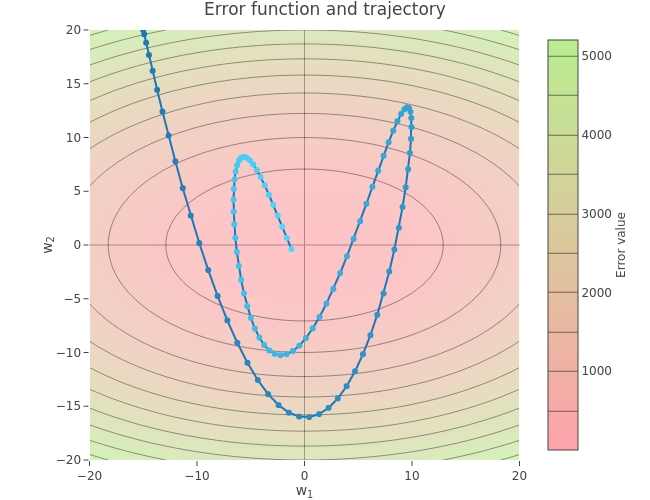
\includegraphics[width=0.8\textwidth]{trajectory.png}
                  \caption{Oszillation durch zu großen Momentumfaktor}
                \end{figure}

          \item Geeignete Parameter sind z.B. $\eta = 0.02$ und $\alpha = 0.5$, nach 20 iterationen beträgt der Fehler $0.0028$:
                \begin{figure}[H]
                  \centering
                  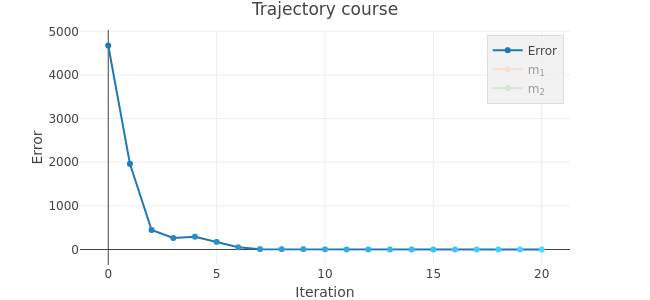
\includegraphics[width=0.8\textwidth]{13d_error.png}
                  \caption{Fehler bei geeigneter Parameterwahl}
                \end{figure}
        \end{enumerate}

\end{enumerate}

\section{Adaptive Learning Rates}
\begin{enumerate}
  \item (siehe Jupyter Notebook)
  \item
        \begin{enumerate}[label=\alph*)]
          \item Einfluss von $\sqrt{s(t) + \epsilon}$: \\\\
                \begin{tabular}{c|cc}
                  \toprule
                  Problem                      & $\displaystyle \sqrt{s(t) + \epsilon} < 1$ & $\sqrt{s(t) + \epsilon} > 1$ \\
                  \midrule
                  \textit{vanishing gradients} & wird gemildert                             & wird verstärkt               \\
                  \textit{exploding gradients} & wird verstärkt                             & wird gemildert               \\
                  \bottomrule
                \end{tabular}
          \item Angenommen, das \textit{exploding gradient} Problem tritt auf, und es gilt $\sqrt{s(t) + \epsilon} < 1$,
                wird $s(t)$ in nachfolgenden Schritten auch erhöht (da $s(t+1)$ abhängig von $\nabla E(w(t))$),
                sodass in nachfolgenden Iterationen gilt $\sqrt{s(t) + \epsilon} > 1$,
                was das \textit{exploding gradient} Problem mildert.
                Analog im Fall \textit{vanishing gradient}.
        \end{enumerate}
  \item
        \begin{enumerate}[label=\alph*)]
          \item $\beta = 0, \quad \epsilon = 0$
                \begin{align*}
                   & s(t) = \nabla E(w(t-1))^2                                                        \\
                   & \implies w(t) = w(t-1) - \eta \frac{\nabla E(w(t-1))}{\sqrt{\nabla E(w(t-1))^2}} \\
                   & \implies w(t) = w(t-1) - \eta \sgn(\nabla E(w(t-1)))
                \end{align*}
          \item (Plot siehe Jupyter Notebook)\\
                In diesem Fall wird $w$ immer nur um $\eta$ in Richtung des Minimums verändert.
          \item Die Updates können sich in jeder Komponente nur um 1, $-1$ oder 0 ändern. Dies entspricht einem Schritt parallel zu X bzw. Y Achse oder diagonale Bewegung, wobei die Schrittweite in jede Achsenrichtung 1 oder 0 beträgt.
        \end{enumerate}
  \item
        \begin{enumerate}[label=\alph*)]
          \item $\beta = 0$ und $\epsilon = 0$
                \begin{align*}
                   & \implies s(1) = g_1^2 \quad \wedge \quad s(2)=g_2^2 \\
                   & \implies C_a(-2,2) = -1
                \end{align*}
          \item
                \begin{enumerate}[label=\roman*)]
                  \item Die Bedeutung der Magnitude kann anhand der Ausdehnung der Grafik in $g_2$ Richtung erkannt werden: Für $\beta = 0$ ist neben der Unabhängigkeit von $g_1$ erkennbar, dass der Betrag des Gradienten normiert wird, die Veränderung beträgt $-(g_2 - 1)$. Für größere $\beta$ ist eine stärkere Verstärkung kleiner Gradienten erkennbar.
                  \item Die Normalisierungseigenschaft lässt vermuten, dass nahe des Ursprungs der Grafik eine Verstärkung des Gradienten und am Rand der Grafik eine Abschwächung zu erkennen ist. Dies bestätigt sich in der Grafik.
                \end{enumerate}
        \end{enumerate}
  \item
        \begin{enumerate}[label=\alph*)]
          \item
                Mit steigendem $\beta$, steigt die Gewichtung der Magnitude. Vorherige $s(t-1),\ s(t-2), \ \dots,\ s(t-j)$ werden also stärker gewichtet, $s(t)$ ändert sich dadurch langsamer.
          \item Der Gradient zeigt initial in negative $w_2$ Richtung, wodurch $s_2$ ansteigt. Über die weiteren Iterationen bleibt der Gradient in der 2. Komponente betragsmäßig größer, $s_2$ bleibt also auch größer als $s_1$ um den Gradienten zu normalisieren.
          \item Der Pfad läuft zielstrebiger ins Minimum, da nicht durch große Schrittweiten vom optimalen Pfad abgewichen wird, was beim momentum Verfahren besonders bei großem Parameter $\alpha$ vorkommt.
          \item Für den Startpunkt $w=\begin{pmatrix} -17 \\ 1.5 \end{pmatrix}$ liegt $s_1$ größtenteils über $s_2$.
        \end{enumerate}
\end{enumerate}

\end{document}
